%% abtex2-modelo-trabalho-academico.tex, laurocesar
%% Copyright 2012-2015 by abnTeX2 group at http://www.abntex.net.br/
%%
%% This work may be distributed and/or modified under the
%% conditions of the LaTeX Project Public License, either version 1.3
%% of this license or (at your option) any later version.
%% The latest version of this license is in
%%	http://www.latex-project.org/lppl.txt
%% and version 1.3 or later is part of all distributions of LaTeX
%% version 2005/12/01 or later.
%%
%% This work has the LPPL maintenance status `maintained'.
%%
%% The Current Maintainer of this work is the abnTeX2 team, led
%% by Lauro César Araujo. Further information are available on
%% http://www.abntex.net.br/
%%
%% This work consists of the files abntex2-modelo-trabalho-academico.tex,
%% abntex2-modelo-include-comandos and abntex2-modelo-references.bib
%%

% ------------------------------------------------------------------------
% ------------------------------------------------------------------------
% abnTeX2: Modelo de Trabalho Academico (tese de doutorado, dissertacao de
% mestrado e trabalhos monograficos em geral) em conformidade com
% ABNT NBR 14724:2011: Informacao e documentacao - Trabalhos academicos -
% Apresentacao
% ------------------------------------------------------------------------
% ------------------------------------------------------------------------

\documentclass[
	% -- opções da classe memoir --
	12pt,				% tamanho da fonte
	openright,			% capítulos começam em pág ímpar (insere página vazia caso preciso)
	oneside,			% para impressão em verso e anverso. Oposto a oneside
	a4paper,			% tamanho do papel.
	% -- opções da classe abntex2 --
	chapter=TITLE,		% títulos de capítulos convertidos em letras maiúsculas
	%section=TITLE,		% títulos de seções convertidos em letras maiúsculas
	%subsection=TITLE,	% títulos de subseções convertidos em letras maiúsculas
	%subsubsection=TITLE,% títulos de subsubseções convertidos em letras maiúsculas
	% -- opções do pacote babel --
	english,			% idioma adicional para hifenização
	french,				% idioma adicional para hifenização
	spanish,			% idioma adicional para hifenização
	brazil				% o último idioma é o principal do documento
	]{abntex2}

% Pacotes básicos
\usepackage{helvet}			% Usa a fonte Latin Modern - Mudei para Helvetica
\usepackage[T1]{fontenc}		% Selecao de codigos de fonte.
\usepackage[utf8]{inputenc}	% Codificacao do documento (conversão automática dos acentos)
\usepackage{lastpage}		% Usado pela Ficha catalográfica
\usepackage{indentfirst}		% Indenta o primeiro parágrafo de cada seção.
\usepackage{color}			% Controle das cores
\usepackage{graphicx}		% Inclusão de gráficos
\usepackage{microtype} 		% para melhorias de justificação


% Pacotes adicionais, usados apenas no âmbito do Modelo Canônico do abnteX2
\usepackage{lipsum}				% para geração de dummy text
\usepackage{customizacoes} 		% customizações feitas pelo autor

% Pacotes de citações
\usepackage[brazilian,hyperpageref]{backref}	% Paginas com as citações na bibl
\usepackage[alf]{abntex2cite}				% Citações padrão ABNT


% CONFIGURAÇÕES DE PACOTES
% Configurações do pacote backref
% Usado sem a opção hyperpageref de backref
\renewcommand{\backrefpagesname}{ }
% Texto padrão antes do número das páginas
\renewcommand{\backref}{\ABNTEXchapterfont}
% Define os textos da citação
\renewcommand*{\backrefalt}[4]{
	\ifcase #1 %
		%
	\or
		%
	\else
		%
	\fi}%

% Informações de dados para CAPA e FOLHA DE ROSTO
\titulo{Habilitando um Prédio a Localizar Contextualmente Dispositivos utilizando Redes Sem Fio}
\autor{Luís Henrique Puhl de Souza}
\local{Bauru}
\data{2016}
\orientador{Prof. Dr. Eduardo Martins Morgado}

\instituicao{%
  Universidade Estadual Paulista ``Júlio de Mesquita Filho''
  %\par
  Faculdade de Ciências - Campus Bauru
  %\par
  Departamento de Computação
}
\tipotrabalho{Monografia (Trabalho de Conclusão de Curso)}
% O preambulo deve conter o tipo do trabalho, o objetivo,
% o nome da instituição e a área de concentração
\preambulo{ Projeto de Trabalho de Conclusão de Curso de Bacharelado em Ciência
da Computação da Universidade Estadual Paulista ``Júlio de Mesquita Filho'',
Faculdade de Ciências, Campus Bauru }

% Configurações de projeto
\newif\iffinal
\finalfalse % define se é um arquivo final, se for não for retira umas partes.

\newif\ifabstract
\abstractfalse % define se mostra o abstract em inglês ou não.

% Configurações de aparência do PDF final
% alterando o aspecto da cor azul
\definecolor{blue}{RGB}{0,0,0}

% informações do PDF
\makeatletter
\hypersetup{
	  	%pagebackref=true,
		pdftitle={\@title},
		pdfauthor={\@author},
	 	pdfsubject={\imprimirpreambulo},
		 pdfcreator={LaTeX with abnTeX2},
		pdfkeywords={beacon}{raspberry pi}{internet das coisas}{abntex2}{trabalho acadêmico},
		colorlinks=true,		 		% false: boxed links; true: colored links
	 	linkcolor=blue,			 	% color of internal links
	 	citecolor=blue,		  		% color of links to bibliography
	 	filecolor=magenta,				% color of file links
		urlcolor=blue,
		bookmarksdepth=4
}
\makeatother

% Espaçamentos entre linhas e parágrafos
% O tamanho do parágrafo é dado por:
\setlength{\parindent}{1.3cm}

% Controle do espaçamento entre um parágrafo e outro:
\setlength{\parskip}{0.2cm}  % tente também \onelineskip

% compila o indice
\makeindex

% Início do documento
\begin{document}

% Seleciona o idioma do documento (conforme pacotes do babel)
%\selectlanguage{english}
\selectlanguage{brazil}

% Retira espaço extra obsoleto entre as frases.
\frenchspacing

% ----------------------------------------------------------
% ELEMENTOS PRÉ-TEXTUAIS
% ----------------------------------------------------------
\pretextual

\ABNTEXchapterfont {

% Capa
\imprimircapa

% Folha de rosto
% (o * indica que haverá a ficha bibliográfica)
%\imprimirfolhaderosto

% Inserir a ficha bibliografica

% Isto é um exemplo de Ficha Catalográfica, ou ``Dados internacionais de
% catalogação-na-publicação''. Você pode utilizar este modelo como referência.
% Porém, provavelmente a biblioteca da sua universidade lhe fornecerá um PDF
% com a ficha catalográfica definitiva após a defesa do trabalho. Quando estiver
% com o documento, salve-o como PDF no diretório do seu projeto e substitua todo
% o conteúdo de implementação deste arquivo pelo comando abaixo:
%
% \begin{fichacatalografica}
%	  \includepdf{fig_ficha_catalografica.pdf}
% \end{fichacatalografica}

\iffinal
  \begin{fichacatalografica}
	\sffamily
	\vspace*{\fill}					% Posição vertical
	\begin{center}					% Minipage Centralizado
	\fbox{\begin{minipage}[c][8cm]{13.5cm}		% Largura
	\small
	\imprimirautor
	%Sobrenome, Nome do autor

	\hspace{0.5cm} \imprimirtitulo  / \imprimirautor. --
	\imprimirlocal, \imprimirdata-

	\hspace{0.5cm} \pageref{LastPage} p. : il. (algumas color.) ; 30 cm.\\

	\hspace{0.5cm} \imprimirorientadorRotulo~\imprimirorientador\\

	\hspace{0.5cm}
	\parbox[t]{\textwidth}{\imprimirtipotrabalho~--~\\ \imprimirinstituicao,
	\imprimirdata.}\\

	\hspace{0.5cm}
		2. Internet das Coisas.
		I. \imprimirorientador.
		II. Universidade Estadual Paulista ``Júlio de Mesquita Filho''.
		III. Faculdade de Ciências.
		IV. Título
	\end{minipage}}
	\end{center}
  \end{fichacatalografica}
\fi

% INSERIR ERRATA
%\begin{errata}
%Elemento opcional da \citeonline[4.2.1.2]{NBR14724:2011}. Exemplo:

%\vspace{\onelineskip}

%FERRIGNO, C. R. A. \textbf{Tratamento de neoplasias ósseas apendiculares com
%reimplantação de enxerto ósseo autólogo autoclavado associado ao plasma
%rico em plaquetas}: estudo crítico na cirurgia de preservação de membro em
%cães. 2011. 128 f. Tese (Livre-Docência) - Faculdade de Medicina Veterinária e
%Zootecnia, Universidade de São Paulo, São Paulo, 2011.

%\begin{table}[htb]
%\center
%\footnotesize
%\begin{tabular}{|p{1.4cm}|p{1cm}|p{3cm}|p{3cm}|}
%  \hline
%	\textbf{Folha} & \textbf{Linha}  & \textbf{Onde se lê}  & \textbf{Leia-se}  \\
%	 \hline
%	 1 & 10 & auto-conclavo & autoconclavo\\
%	\hline
%\end{tabular}
%\end{table}

%\end{errata}


% INSERIR FOLHA DE APROVAÇÃO
% Isto é um exemplo de Folha de aprovação, elemento obrigatório da NBR
% 14724/2011 (seção 4.2.1.3). Você pode utilizar este modelo até a aprovação
% do trabalho. Após isso, substitua todo o conteúdo deste arquivo por uma
% imagem da página assinada pela banca com o comando abaixo:
%
% \includepdf{folhadeaprovacao_final.pdf}
%
\begin{folhadeaprovacao}
  \ABNTEXchapterfont {

	 \begin{center}

		{\ImprimirAutor}

		\vspace*{\fill}\vspace*{\fill}

		\begin{center}
		  \bfseries\large\ImprimirTitulo
		\end{center}

		\vspace*{\fill}

		\hspace{.45\textwidth}
		\begin{minipage}{.5\textwidth}
			 \imprimirpreambulo
		\end{minipage}%
		\vspace*{\fill}
	  \end{center}

	  %Trabalho aprovado. \imprimirlocal, 24 de novembro de 2012:

	  %\assinatura{\textbf{\imprimirorientador} \\ Orientador}
	  %\assinatura{\textbf{\imprimircoorientador} \\ Coorientador}
	  %\assinatura{\textbf{Professor} \\ Convidado 1}
	  %\assinatura{\textbf{Professor} \\ Convidado 2}
	  %\assinatura{\textbf{Professor} \\ Convidado 3}
	  %\assinatura{\textbf{Professor} \\ Convidado 4}
		\vspace*{0.5cm}
		\hspace{.5\textwidth}
	  \begin{center}
		 \ImprimirLocal \\ \imprimirdata
	  \end{center}
  }
\end{folhadeaprovacao}

% DEDICATÓRIA
\iffinal
  \begin{dedicatoria}
	\vspace*{\fill}
	\centering
	\noindent
	\textit{} \vspace*{\fill}
  \end{dedicatoria}
\fi

% AGRADECIMENTOS
\iffinal
	\begin{agradecimentos}
	\end{agradecimentos}
\fi

% EPÍGRAFE
\iffinal
  \begin{epigrafe}
	 \vspace*{\fill}
	\begin{flushright}
		\textit{}
	\end{flushright}
  \end{epigrafe}
\fi

% RESUMOS
\ifabstract
% RESUMO EM PORTUGUÊS
\setlength{\absparsep}{18pt} % ajusta o espaçamento dos parágrafos do resumo
\begin{resumo}
	\ABNTEXchapterfont {
		\textbf{Palavras-chave}: IoT. Internet das Coisas. GPS de interiores. Posicionamento Contextual.
	}
\end{resumo}

% RESUMO EM INGLÊS
\begin{resumo}[Abstract]
	\begin{otherlanguage*}{english}
		This is the english abstract.
		\vspace{\onelineskip}
		\noindent
		\textbf{Keywords}: IoT. Indoor GPS. Contextual Positioning.
	 \end{otherlanguage*}
\end{resumo}
\fi

% INSERIR LISTA DE ILUSTRAÇÕES
\iffinal
  \pdfbookmark[0]{\listfigurename}{lof}
  \listoffigures*
  \cleardoublepage
\fi

% INSERIR LISTA DE TABELAS
\iffinal
  \pdfbookmark[0]{\listtablename}{lot}
  \listoftables*
  \cleardoublepage
\fi

% INSERIR LISTA DE ABREVIATURAS E SIGLAS
\iffinal
  \begin{siglas}
	 \item[ANN] \textit{Artificial Neural Networks}
  \end{siglas}
\fi

% INSERIR LISTA DE SÍMBOLOS
\iffinal
  \begin{simbolos}
	 \item[$ \Gamma $] Letra grega Gama
	 \item[$ \Lambda $] Lambda
	 \item[$ \zeta $] Letra grega minúscula zeta
	 \item[$ \in $] Pertence
  \end{simbolos}
\fi

% INSERIR O SUMARIO
\pdfbookmark[0]{\contentsname}{toc}
\tableofcontents*
\cleardoublepage


% ------------------------------------------------------------------------------
% ELEMENTOS TEXTUAIS
% ------------------------------------------------------------------------------
\textual

\chapter[INTRODUÇÃO]{INTRODUÇÃO}
%\addcontentsline{toc}{chapter}{Introdução}

Recentemente, Internet das Coisas (IoT - \textit{Internet of Things}) vem
tomando o foco das atenções de empresas e entusiastas de Tecnologia da
Informação \cite{DzoneIoT:2015} a tal
ponto que as empresas líderes do segmento já incluem IoT como uma de suas áreas
de atuação \cite{Ibm2016} \cite{ARM-mbed} \cite{Microsoft2016} \cite{Intel2016}
\cite{Oracle2016} \cite{Google2016} \cite{AmazonIoT2016}.

Todo este movimento no mercado é justificado pelo baixo custo dos pequenos
dispositivos computacionais \cite{RpiZeroLaunch} \cite{Esp8266.net} e grandes
serviços na nuvem \cite{Kaufmann2015} \cite{Amazon2016}. Este baixo custo
possibilita a computação ubíqua descrita por Weiser em 1991 e 1992
\cite{Weiser1999} que é entendida pelos autores como \textit{``computação
virtualmente onipresente''}. Também para os autores, esta virtual onipresença é
base e consequência para a IoT, sendo esta a realizadora da computação ubíqua.

Uma vez contextualizado o mercado e a oportunidade de implementação da
computação ubíqua, percebemos a necessidade de dar aos elementos cotidianos
(coisas) a capacidade info-computacional, tornando-os sensores e atuadores
conectados, unicamente identificáveis e acessíveis através da rede mundial
de computadores \cite{Lemos2013} \cite{Kranenburg2012}.

É esperado que uma quantia total de 6,4 bilhões de dispositivos conectados
exista até o final de 2016 \cite{GARTNER2015} e entre 26 bilhões
\cite{GARTNER2014} e 50 bilhões até 2020 com até 250 novas coisas conectando-se
por segundo \cite{CiscoBlog2013}.

\chapter{PROBLEMA}
\label{chap:PROBLEMA}

Tamanha quantidade de dispositivos conectados pouco acrescenta na vida diária se
humanos ou coisas não puderem simplesmente se encontrar, tanto em ambiente real
quanto virtual é necessário o contato entre as partes para a existência de uma
interação.

Mais ainda, para melhor funcionamento de aplicações como o uso de conteúdo
específico para cada usuário e situação é necessário coletar informações
contextuais. Para a maioria das aplicações, a informação contextual de maior
relevância é a localização física.

Destacamos a necessidade da criação desta informação através de sensores ativos
sempre que necessário para que o dispositivo tenha ciência deste contexto em
suas tomadas de decisão e para que outros (sistemas, pessoas e coisas) saibam a
localização de qualquer dispositivo ao qual têm interesse de interagir.

Um exemplo da necessidade de localização de dispositivos dentro de um prédio
seria um profissional saber onde está o dispositivo em seu local de trabalho,
seja ele um vendedor e seu tablet para demostrar um produto fora de estoque em
uma loja ou um médico e um desfibrilador.

\section{SOBRE SISTEMAS DE POSICIONAMENTO}
\label{sec:SOBRE SISTEMAS DE POSICIONAMENTO}

Sistemas de posicionamento (PS - \textit{Positioning System}) são geralmente
constituídos de um Ponto Origem Global escolhido (\textit{O}) e um conjuto não
vazio de Pontos de Referência (RP - \textit{Reference Point}) cuja localização
global em relação ao \textit{O} é conhecida com precisão maior ou igual a
oferecida pelo sistema.

Também faz parte do sistema o ponto móvel (MU - \textit{Mobile User}) sobre o
qual temos interesse em determinar a posição que é feita pelo PS encontrando uma
distância (com dimensão variável de acordo com o método utilizado para
adquirir a distância) relativa a um sub-conjunto de RPs. Feito isso, é possível utilizar
modelos matemáticos para, a partir das distâncias, encontrar uma posição do MU
em relação aos RPs e uma nova transformação é aplicada para encontrar a posição
relativa ao \textit{O}.

Uma das maneiras de classificar PSs é entre os de Auto Posicionamento e
Posicionamento Remoto. Os de Auto Posicionamento contém no MU todo aparato
necessário para medir a distância dos RPs e calcular a posição em relação a
\textit{O}. Já os de Posicionamento Remoto tem o mínimo necessário na MU e todo
o trabalho de cálculo de distância e posição global é feito nos RPs ou em uma
unidade coordenadora destes.

Para PSs eletrônicos baseados em radio-frequência (RF - \textit{Radio
Frequency}), geralmente, utilizam-se dois componentes básicos, Transmissores e
Receptores, os quais assume-se que ao menos um destes está no RP e ao menos um
outro no MU. Para calcular a distância entre MU e RP, utiliza-se as propriedades
da comunicação por RF como tempo de chegada (TOA - \textit{Time Of Arrival}),
diferencial de tempo de chegada (TDOA - \textit{Time Difference Of Arrival}) e
ângulo de chegada de sinal (AOA - \textit{Angle Of Arrival}).

Para maior precisão, é comum a utilização de múltiplas RPs geralmente com o
número mínimo igual ao número de dimensões espaciais que deseja-se calcular.
Notamos que para sistemas distribuídos a sincronização de relógios é um problema
clássico então o tempo conta como dimensão.

Os sistemas classificados como ``Sistema de Navegação Global por Satélite''
(GNSS - \textit{Global Navigation Satellite System}), como o tradicional
Estadunidense Sistema de Posicionamento Global (GPS - \textit{Global Positioning
System}), utilizam a técnica em que o dispositivo móvel contém o receptor e os
transmissores são fixos em satélites na órbita terrestre \cite{Djuknic2001}.
Devido a posição e número de satélites, o GPS e seus correlatos estão sempre
presentes do ponto de vista de um observador da superfície terrestre, sendo para
este tipo de usuário um sistema ubíquo.

Entretanto, a força do sinal GNSS não é suficiente para penetrar a maioria dos
prédios, uma vez que estes dependem de visão direta (LOS -
\textit{Line-Of-Sight}) entre os satélites e o receptor. A reflexão do sinal
muitas vezes permite a leitura em ambientes fechados, porém o cálculo da posição
não será confiável \cite{Dartmouth2000}. Portanto, apesar da ubiquidade dos
GNSSs em ambientes abertos, são necessárias soluções diferentes para obter um
Sistema de Posicionamento para Ambientes Fechados (IPS - \textit{Indoor
Positioning System}) sendo a ubiquidade deste essencial para conquistar o mesmo
nível de confiança trazido pelos GNSSs.

Para implementar este IPS, propomos o uso de tecnologias já implantadas em
dispositivos móveis e essenciais para o funcionamento dos mesmos, especialmente
as de camadas de comunicação, que são ubíquas no ambiente dos dispositivos
móveis, como Wi-Fi (padrão \textit{IEEE 802.11}) e Bluetooth (padrão \textit{Bluetooth
SIG}), para que os objetos conectados em que temos interesse de encontrar o
contexto locativo não necessitem de modificações.

\chapter{JUSTIFICATIVA}
\label{chap:JUSTIFICATIVA}

Nossa proposta de IPS é de Posicionamento Remoto localizando dentro de um
ambiente fechado dispositivos conectados a internet (IoT Devices) através de
redes Wi-Fi e Bluetooth. Mediremos a distância destes MUs (devices) aos RP
(sensores) utilizando o resíduo eletromagnético das redes sem fio
(\textit{sniffing}) disponibilizando as informações encontradas através de uma
REST WEB API.

Sobre o contexto encontrado, propomos um ambiente consciente onde o contexto
locativo oriundo do posicionamento remoto de cada dispositivo móvel é
administrado e divulgado pelo prédio conectado ao invés da auto localização do
aparelho, pois:

\begin{alineas}

	\item Uma vez encontrada a localização, é mais fácil propagar esta informação do
ambiente para o aparelho em comparação ao auto posicionamento, pois a negociação
entre o ambiente e o aparelho é nula quando o primeiro contém a informação- o
ambiente sempre disponibilizará uma informação coletada para o gerador desta
informação;

	\item Pode-se lidar com grande heterogeneidade de dispositivos, uma vez
que cada um deles não precisa se adaptar para cada mudança de ambiente;

	\item Este tipo de informação já é contida nos históricos de cada Ponto de
	Acesso Wi-Fi (AP - \textit{Access Point}), porém:

	\begin{alineas}

		\item Geralmente sem uso - poucas são as aplicações que usam a
		localização obtida pelo AP;

		\item Com granularidade insuficiente para uso em aplicações
		contextualizadas;

		\item geralmente não disponibilizada pelos APs.

	\end{alineas}

	\item Uma vez instalado um PS deste gênero, a quantia de dispositivos que
	ele pode localizar fica limitada apenas pela rede física;

	\item Economia de hardware quando menos é exigido de cada dispositivo.

\end{alineas}

Levamos em conta também a quantidade prevista de em média 5 dispositivos IoT
por pessoa que seriam beneficiados sempre que utilizados no ambiente conectado.

\begin{figure}[htb]
	\caption{\label{fig:projeto}Modelo das camadas }
	\begin{center}
		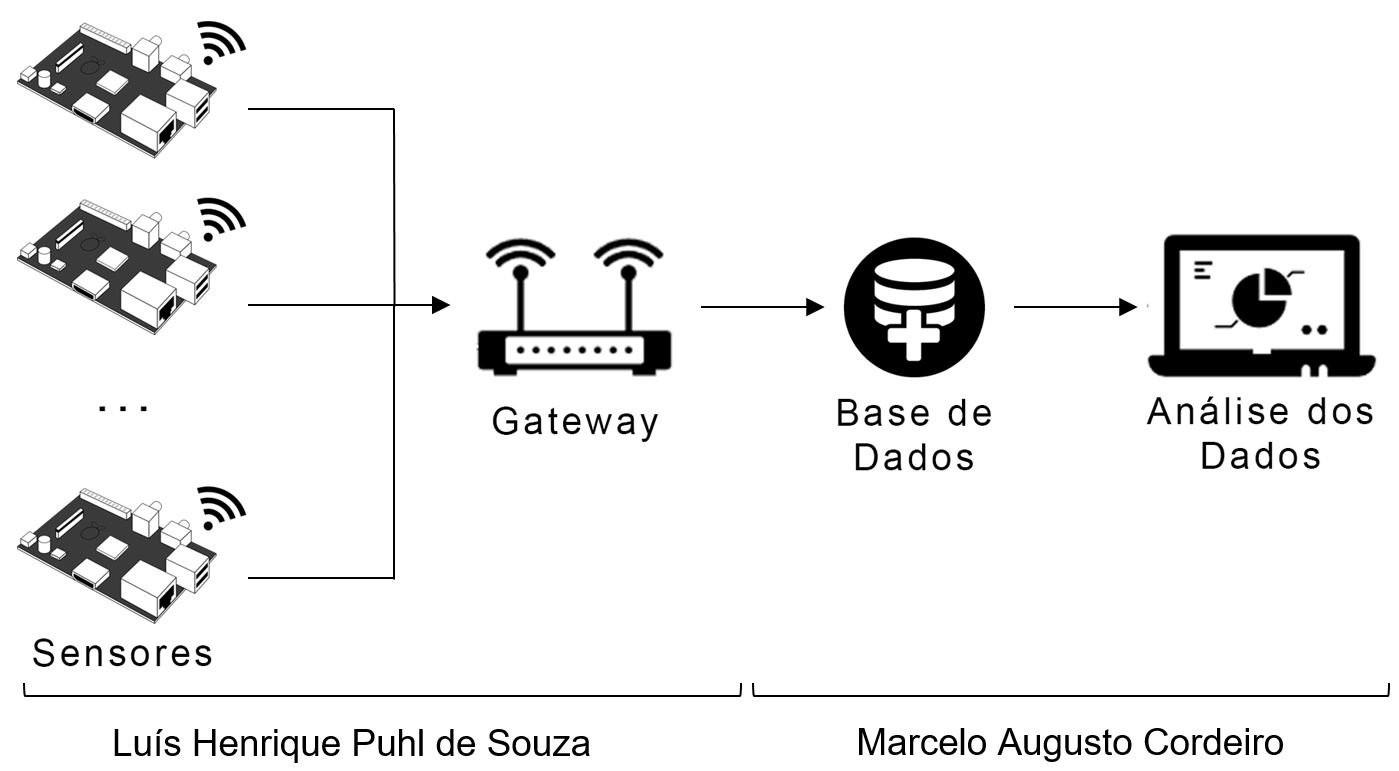
\includegraphics[width=1\textwidth]{img/projeto.JPG}
	\end{center}
	\legend{Fonte: Marcelo Augusto Cordeiro}
\end{figure}

A Figura \ref{fig:projeto} apresenta a arquitetura simplificada de uma aplicação
IoT.

Para possibilitar testes em um ambiente real, o projeto aqui proposto será
instalado dentro do prédio do Laboratório de Tecnologia da Informação Aplicada
(LTIA) da Faculdade de Ciências da Unesp de Bauru.

\chapter{OBJETIVOS}
\label{chap:OBJETIVOS}

\section{OBJETIVO GERAL}
\label{sec:OBJETIVO GERAL}

Considerando características locais, propõem-se a construção de uma aplicação
para localizar contextualmente dispositivos dentro de um prédio piloto e avaliar
sua precisão.

Além desta aplicação, é objetivo definir o custo do projeto piloto, incluindo
esforço de pesquisa assim como definir um custo para replicação deste
localizador contextual em outros prédios.

\section{OBJETIVOS ESPECÍFICOS}
\label{sec:OBJETIVOS ESPECÍFICOS}

\begin{alineas}

	\item Estabelecer o estado da arte sobre a desenvolvimento de aplicações IoT;

	\item Identificar desafios locais para o desenvolvimento;

	\item Identificar provedores de serviços, dispositivos e ferramentas para o
desenvolvimento;

	\item construir sensores de identificação e localização (distância) de
 dispositivos cuja comunicação seja baseada em Bluetooth e Wi-Fi;

	\item Posicionar estes sensores;

	\item Construir um dispositivo agregador de informações dos sensores
 (\textit{gateway}) e sua interface web (Web REST API - \textit{Representational
State Transfer} \textit{Application Programming Interface});

	\item Estimar o custo total do projeto piloto incluindo esforço de pesquisa;

	\item Estimar o custo de replicação da aplicação em outros prédios.

\end{alineas}

\chapter{MÉTODO DE PESQUISA}
\label{chap:MÉTODO DE PESQUISA}

Abordagens para medir distâncias através de redes sem fio Wi-Fi
\cite{bahillo2009ieee} e Bluetooth já existem e, propor novas maneiras não é o
foco deste trabalho. Utilizando essas técnicas, propomos estabelecer uma rede de
nós sensores colaborativos fixos no ambiente onde deseja-se obter a localização
dos dispositivos. As informações de distância serão compartilhadas entre os nós
para maior precisão da informação.

Para a implementação, pretende-se utilizar os softwares de maior destaque
recentemente nos ramos de comunicação de baixa energia (\textit{MQTT}), serviços
\textit{Web} para armazenamento (\textit{MongoDB}) e publicação
(\textit{NodeJS}), além de softwares para medição da distância sem interferir na
comuncação (\textit{Sniffing}) e das plataformas de hardware disponíveis e
recomendadas para IoT com capacidade Wi-Fi e Bluetooth (\textit{Raspberry Pi
3}).

Mesmo com a grande quantidade de dispositivos já conectados são poucos os
documentos descrevendo boas práticas para concepção, construção e manutenção de
aplicações IoT, especialmente sobre os cuidados tomados quanto a segurança e
análise de custos para a implementação e manutenção.

Além disso, a falta de referências neste sentido é agravada quando considera-se
a implementação no interior do estado de São Paulo. Nesta região, poucas são as
organizações atualizadas neste tema, levando a uma falta enorme de conteúdo
escrito na linguagem local além de serviços e produtos disponíveis para
construção de uma plataforma completa e competitiva nesta região.

Devido a falta de conteúdo e instrução, utilizaremos prototipagem ágil para este
projeto, uma vez que esta metodologia de desenvolvimento é recomendada para
projetos cujas especificações e definições não são claras, demandando muitas
modificações das mesmas durante a execução do mesmo. Esse método entra em
contraste com metodologias clássicas, como a cascata que apesar de previsíveis,
não reagem bem a ambientes de extrema incerteza.

Mais especificamente, utilizaremos uma variante da metodologia \textit{Scrum}
\cite{James2016} que será adaptada para o projeto. Nela, serão executadas
iterações de uma semana em que a cada iteração, uma nova versão melhorada do
produto completo (hardware, software, documentação e resultados) será entregue.

Dentro de cada iteração, as camadas da aplicação IoT serão escolhidas,
implementadas, justificadas e avaliadas, sendo todo processo documentado. Como
resultado de cada uma delas, será gerado um relatório das mudanças a partir da
iteração anterior.

Com mais detalhes, cada iteração cumprirá uma parte de cada objetivo no trabalho
completo levando o projeto integralmente para um estágio de completude maior a
cada iteração. Serão foco de cada iteração os objetivos abaixo, gerando um
relatório utilizado para tomar e justificar decisões durante a execução do
projeto bem como servir de posterior documentação. Os objetivos de cada iteração
são:

\begin{alineas}

	\item Escolha de provedores de serviços, dispositivos e ferramentas para o
desenvolvimento;

	\item construir, avaliar, testar e manter dos sensores;

	\item construir um dispositivo agregador e sua API;

	\item Estimar o custo total do projeto piloto;

	\item Estimar o custo de replicação;

	\item Identificar os desafios para o desenvolvimento.

\end{alineas}

Desta forma, esperamos garantir a liberdade necessária para o projeto ser
executado com sucesso, mesmo no ambiente de incerteza no qual o mercado local de
IoT encontra-se, cumprindo as premissas de de funcionamento, manutenção e
segurança que são grande importância para os interessados na área.


\chapter{CRONOGRAMA}
\label{chap:CRONOGRAMA}

Devido a natureza ágil e iterativa da metodologia, o cronograma será dividido em
apenas três partes: Levantamento Bibliográfico Inicial, Desenvolvimento
Iterativo (Escolha de provedores e fornecedores; Construção, avaliação, teste e
manutenção dos sensores e agregadores; Estimativas de custos totais e de
replicação e Documentação de desenvolvimento) e Revisão Final. Estas partes
serão distribuídas conforme a Tabela 1.

\begin{table}[htb]
\IBGEtab{%
\ABNTEXchapterfont {
  \caption{Cronograma de Atividades Propostas}%
  \label{table:cronograma}
}
}{%
  \begin{tabular}{cccccccccc}
  \toprule
	Atividade															&	Fev	&	Mar	&	Abr	&	Mai	&	Jun	&	Jul	&	Ago	&	Set	&	Out \\
  \midrule \midrule
	Levantamento Bibliográfico Inicial									&	X	&	X	&	 	&	 	&	 	&	 	&	 	&	 	&	  \\
  \midrule
  Escolha de provedores e fornecedores									&	 	&	X	&	X	&	X	&	X	&	X	&		&		&	  \\
  \midrule
  Construção, avaliação e manutenção \\ dos sensores e agregadores	&	 	&		&	X	&	X	&	X	&	X	&	X	&		&	  \\
  \midrule
  Estimativas de custos							&	 	&		&		&		&	X	&	X	&	X	&	X	&	  \\
  \midrule
  Documentação de desenvolvimento										&	 	&		&	X	&	X	&	X	&	X	&	X	&	X	&	  \\
  \midrule
  Revisão Final															&	 	&	 	&	 	&	 	&	 	&	 	&	X 	&	X	&	X \\
  \bottomrule
\end{tabular}%
}{%
  \fonte{Produzido pelo autor.}%
  }
\end{table}

% ----------------------------------------------------------------------------

% ELEMENTOS PÓS-TEXTUAIS


% Referências bibliográficas
\bibliography{referencias}


\end{document}
